\documentclass{article}
% \usepackage{hyperref}

\usepackage{titlesec}
\usepackage{titling}
\usepackage{multicol}
% \usepackage{hyperref}
\usepackage[margin=0.2in]{geometry}

\usepackage{MnSymbol}
\usepackage{amsmath} 
\usepackage{graphicx} 
\usepackage{eso-pic}
\usepackage[hidelinks]{hyperref}

\hypersetup{
    colorlinks=true,
    linkcolor=blue,
    filecolor=magenta,      
    urlcolor=[rgb]{0,0,1},
    pdftitle={Kaustav-Resume},
    % pdfpagemode=FullScreen,
    }


\usepackage{ifthen}
\newboolean{showProjectlinks}
\setboolean{showProjectlinks}{true}


\titleformat{\section}
{\large\uppercase}
{}
{0em}
{}[\titlerule]

\titleformat{\subsection}[runin]
{\bfseries}
{}
{1em}
{}[]

%%%%%%%%%%%%%%%%   Make Title for Heading Style 1  %%%%%%%%%%%%%%%%

% \renewcommand{\maketitle}{
%     \begin{flushleft}        
%         {\huge\rmfamily
%         \theauthor}\newline
%         \vspace{0.1em}
%         \textmd{teetangh@gmail.com -- github.com/teetangh}\newline
%         \textmd{Contact No. -- +91-8800441954}\newline
%         \textmd{Manipal Institute of Technology}\newline
%         \textmd{B.Tech in \textbf{Computer Science \& Engineering}}
%         \textmd{2018 - 2022}\newline
%         \textmd{Minor in \textbf{Computational Intelligence}}\newline
%         \textmd{CGPA: 8.54/10}\newline
%         \href{https://www.github.com/teetangh}{GitHub} \
%         \href{https://www.linkedin.com/in/kaustav-ghosh-1538651bb/}{LinkedIn}
%     \end{flushleft}
% }


\titlespacing*{\subsection}
{0em}
{0em}
{0em}


%%%%%%%%%%%%%%%%%%%%%%%%%%%%%%%%%%%%%%   DOCUMENT  %%%%%%%%%%%%%%%%%%%%%%%%%%%%%%%%%%%%%%


%%%%%%%%%%%%%%%%   Heading Style 1  %%%%%%%%%%%%%%%%

\begin{document}
\thispagestyle{empty}  % for no page numbering

% \begin{multicols}{2}
%     \title{Resume}
%     \author{Kaustav Ghosh}
%     \maketitle
%     \begin{flushright}
%         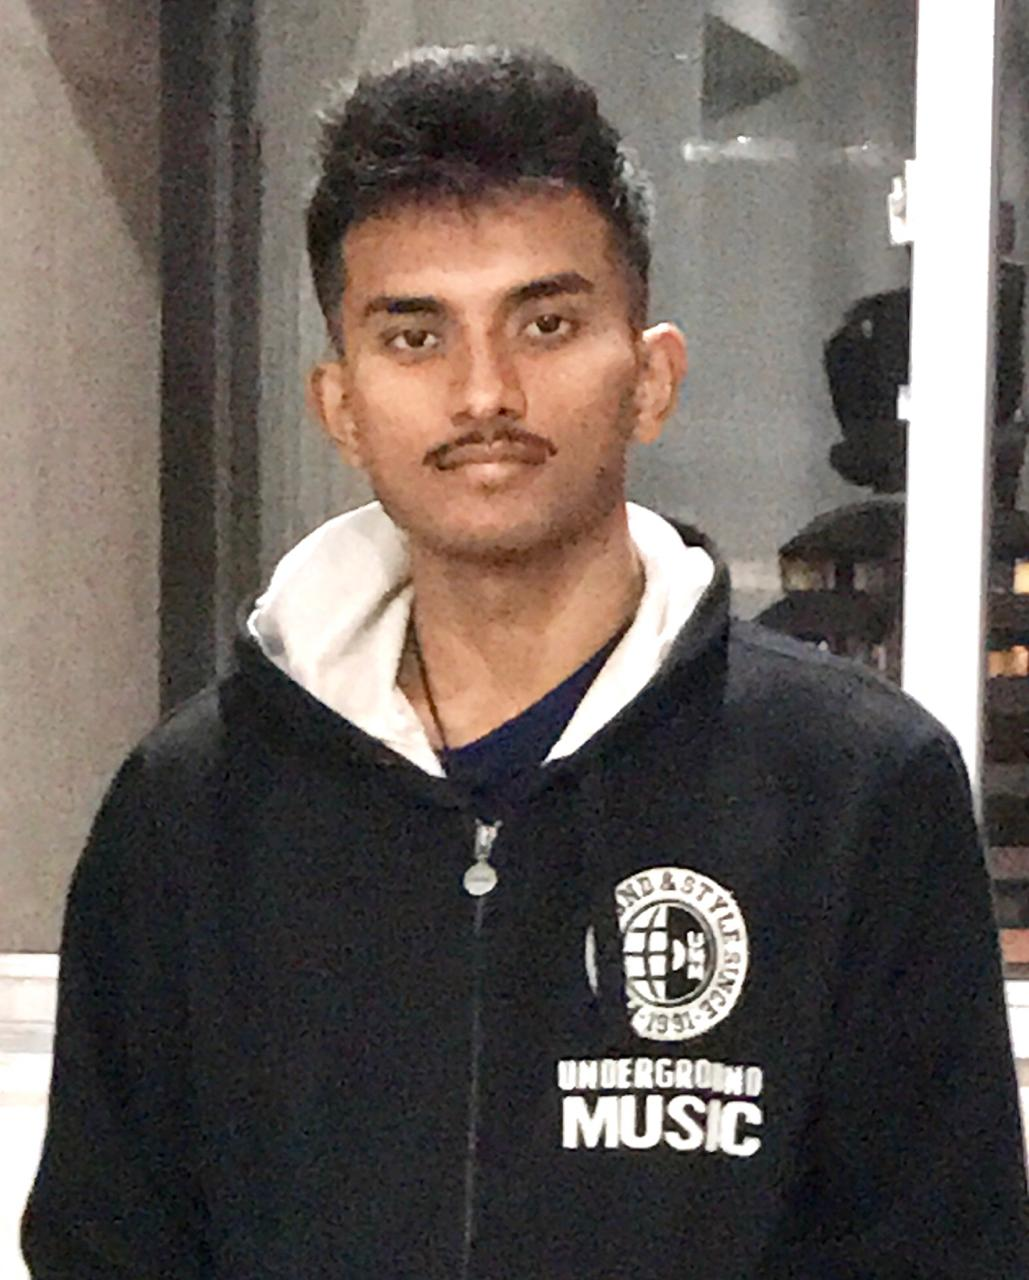
\includegraphics[height=3cm]{kaustav2.jpeg}
%     \end{flushright}
% \end{multicols}


%%%%%%%%%%%%%%%%   Heading Style 2  %%%%%%%%%%%%%%%%

\begin{center}
    \huge{Kaustav Ghosh} % TODO: LEAVE A BLANK LINE AFTER THIS

    \normalsize{
        \textmd{
            \href{https://www.github.com/teetangh}{GitHub} \(|\)
            \href{https://www.linkedin.com/in/kaustav-ghosh-1538651bb/}{LinkedIn} \(|\)
            teetangh@gmail.com \(|\)
            Gugraon,India \(|\)
            +91-8800441954
        }}
\end{center}

%%%%%%%%%%%%%%%%%%%%%%%%%%%%%%%%%%%%%%   Education  %%%%%%%%%%%%%%%%%%%%%%%%%%%%%%%%%%%%%%

\section*{Education}

\textbf{Manipal Institute of Technology} \hfill \textmd{2018-2022}
\textmd{\newline \textmd{BTech in Computer Science \& Engineering specializing in Computational Intelligence}}
% \textmd{\newline \textmd{Interests: Artificial Intelligence and Robotics}}
\ifthenelse{\boolean{showProjectlinks}}{\textbf{Lab Work:}
    \href{https://github.com/teetangh/Kaustav-CSE-LABS-and-Projects}{\text{[Repository]}}.
}{}
\hfill \textmd{CGPA: 8.54/10}



%%%%%%%%%%%%%%%%%%%%%%%%%%%%%%%%%%%%%%   Work Experience  %%%%%%%%%%%%%%%%%%%%%%%%%%%%%%%%%%%%%%

\section*{Work Experience}

\begin{itemize}

    \item{\textbf{\large{Hevo Data, Bangalore - Software Engineer Intern}}} \hfill \textmd{Jan'22-Jun'22}
          \newline
          \textmd{- Designed and implemented an end-to-end connector and SDK for the data source, Braze, a software as a service (SaaS) platform for Customer Engagement by deciding the source objects, the polling strategies, building the SDK authentication, models, client, and the connector offset, tasks, and services for polling each source object. All of this was supplemented by appropriate error handling for Socket Connection and Polling.}
          \newline
          \textmd{- Worked on and resolved several bugs on already existing connectors tracked by Sentry and Coralogix}
          \newline
          \textmd{- Worked on resolving Google Big-Query and Marketo On-call issues supported with Senior developers}
          \newline
          \textmd{- Developed Unit tests for Outbrain.}

    \item{\textbf{\large{Samsung R\&D, Bangalore - Software Engineer Intern, IoT Products \& Analytics}}} \hfill \textmd{Jun'21-Jul'21}
          \newline
          \textmd{- Developed and implemented MQTT bridge functionality in Moquette, an open-source lightweight Java MQTT broker}
          \newline
          \textmd{- Developed a socket programming system for transfer of messages between the MQTT message broker and the bridge client}
          \newline
          \textmd{- Developed a lexical analyzer to parse the user-specified configuration of the bridge properties}

    \item{\textbf{\large{Microsoft Student Partners - Machine Learning Intern}}} \hfill \textmd{Apr'20-Jun'20}
          \newline
          \textmd{- Guided a team of 10 individuals to collaborate and accomplish a Regression task of price prediction of used cars in a machine learning pipeline through Exploratory Data Analysis,Feature Engineering and Model Building.}
          \ifthenelse{\boolean{showProjectlinks}}{
              \textbf{Projects:}\href{https://nbviewer.jupyter.org/github/teetangh/Microsoft-Student-Partners-Machine-Learning-Internship/blob/main/MINOR\%20PROJECT/Microsoft_Minor_Project_v2.ipynb}{\text{[Minor]}}.
              \href{https://nbviewer.jupyter.org/github/Microsoft-ML-Internship-Team/Major-Project-Submissions/tree/master/KAUSTAV/}{\text{[Major]}}.
          }{}

          % \item{\textbf{\large{TakenMind Technologies - Data Analytics Intern}}}\hfill \textmd{May'20}
          %       \newline
          %       \textmd{- Worked on analysing Industrial Data, predicting and presenting trends, using techniques such as Exploratory Data Analysis and Data visualisation using Matplotlib and Seaborn.Implemented several barplots, heatmaps, etc on several datasets.Implemented Machine Learning Algorithms (such as Random Forests).Obtained 87\% test accuracy.}
          %       \ifthenelse{\boolean{showProjectlinks}}{\textbf{Source Code:}
          %           \href{https://nbviewer.jupyter.org/github/Kaggle-Workspace/UN-SDG-Takenmind-Internship-IBM-Employee-Attrition/blob/main/Major\%20Assignment/Predicition.ipynb}{\text{[Notebook]}}.
          %       }{}

\end{itemize}


%%%%%%%%%%%%%%%%%%%%%%%%%%%%%%%%%%%%%%   Research Work  %%%%%%%%%%%%%%%%%%%%%%%%%%%%%%%%%%%%%%

\section*{Research Work}
\begin{itemize}
    % \item{\textbf{\large{Samsung - Intelligent Ranking for Dynamic Restoration in Wireless Networks}}} \hfill \textmd{Sep'20-Mar'21}
    \item{\textbf{\large{Samsung PRISM - Machine Learning Intern}}} \hfill \textmd{Sep'20-Mar'21}
          \newline
          \textbf{Intelligent Ranking for Dynamic Restoration of Next Generation Wireless Networks}
          \newline
          \textmd{- Implemented Machine Learning algorithms and Feature Engineering techniques to predict KPI values for eNodeB-s and consequently a ranking system to orderly restore them during network failure.}
\end{itemize}

%%%%%%%%%%%%%%%%%%%%%%%%%%%%%%%%%%%%%%   Projects  %%%%%%%%%%%%%%%%%%%%%%%%%%%%%%%%%%%%%%

\section*{Projects}
\begin{itemize}
    \item{\textbf{\large{Compiler Front-end for subset of C-Language}}}
          % Don't know why indentation is not working
          \newline
          \textmd{- Coded a \textbf{Lexical Analyser} that extracts tokens from a C source file and a \textbf{Symbol Table Generator} to store information of identifiers and functions and a \textbf{Recursive Decent Parser} that semantically parses the grammar for subset of C-Language by analysing the tokens generated.}
          \ifthenelse{\boolean{showProjectlinks}}{
              \href{https://github.com/teetangh/Kaustav-CSE-LABS-and-Projects\#compiler-design-project}{\text{[Demo]}}
              \textbf{Source Code:}
              \href{https://github.com/teetangh/Kaustav-CSE-LABS-and-Projects/blob/main/Sem05-Compiler-Design-LAB/LAB\%2004/lab04_symbol_table_lexical_analyser_complete.c}{\text{[Lexical Analyser + Symbol Table]}}.
              \href{https://github.com/teetangh/Kaustav-CSE-LABS-and-Projects/blob/main/Sem05-Compiler-Design-LAB/LAB\%200789/lab09_RDP_main.c}{\text{[Recursive Decent Parser]}}.
          }{}
    \item{\textbf{\large{Mini Games based on Backtracking}}}
          \newline
          \textmd{- Coded a \textbf{Crossword Solver} that takes a 10*10 grid and word list and outputs a grid with the words accurately filled}
          \newline
          \textmd{- Coded a \textbf{Sudoku Solver} that takes a partially filled 9*9 Sudoku grid and outputs a solution so that every row, column and nine 3x3 sub-grids contains exactly 1 instance of the digits from 1 to 9.}
          \ifthenelse{\boolean{showProjectlinks}}{
              \href{https://github.com/teetangh/Competitive-Programming\#notable-projects}{\text{[Demo]}}
              \textbf{Source Code:}
              \href{https://github.com/teetangh/competitive-programming/blob/main/CodeZen/03\%20Algorithms\%20and\%20Competitive\%20Programming/11\%20Backtracking/prog004crosswordSolver.cpp}{\text{[Crossword Solver]}}.
              \href{https://github.com/teetangh/competitive-programming/blob/main/CodeChef/Public/Code\%20Marathon/sudokuSolver.cpp}{\text{[Sudoku Solver]}}.
          }{}

    \item{\textbf{\large{Noteups - A Lecutre Notes sharing platform}}}
          \newline
          \textmd{- Implemented the frontend using ReactJS and vanilla Redux, Redux Toolkit and RTK Query for state management, Framer Motion for animations and Styled Components for styling, Media Queries for responsive design, Sass for CSS pre-processing and Font Awesome for icons.}
          \newline
          \textmd{- Implemented the backend using NodeJS and ExpressJS for server-side rendering, used MongoDB for NoSQL DB, cloudinary for pdf and metadata storage, and PassportJS for JWT authentication and Social Login.}
          \newline
          %   \textmd{- Created an encrypted PDF-viewer using PDF.js and ReactPDF for PDF rendering.}
          \textmd{- Implemented functionality to synchronize the note products betweeen cloudinary and MongoDB.}
          \newline
          \textmd{- Working on integrating the backend with Stripe,Paypal and Razorpay for subscription payments.}


          % \item{\textbf{\large{Finland Labs \& IIT Roorkee - Time Series Forecasting, Data Analysis and Web Scraping}}}
          %       % Don't know why indentation is not working
          %       \newline
          %       \textmd{- Prepared a complete Data Analysis report on World-wide COVID-19 attack statistics and used the Facebook's fbprophet Time-series Forecasting library to speculate the number of active corona victim cases in the upcoming days.}\newline
          %       \textmd{- Created neural networks from scratch which facilitated in implementing a machine learning model to recognize the function of an XOR gate without explicitly being programmed.}%\newline
          %       %   \textmd{- Trained a Deep Learning model with TF2 and Keras API for MNIST Handwritten digit Recognition}
          %       \ifthenelse{\boolean{showProjectlinks}}{\textbf{Source Code:}
          %           \href{https://nbviewer.jupyter.org/github/teetangh/FinlandLabs-IITR-COVID-19-Analysis/tree/main
          %           }{\text{[Project]}}.
          %       }{}

          % \item{\textbf{\large{Kaggle - Advanced House Price Prediction Regression Techniques}}}
          %       \newline
          %       \textmd{-With 79 explanatory variables describing (almost) every aspect of residential homes in Ames, Iowa, applied feature engineering and machine learning techniques to predict the final price of each home.}
          %       \ifthenelse{\boolean{showProjectlinks}}{\textbf{Repository:}
          %           \href{https://nbviewer.jupyter.org/github/Kaggle-Workspace/House-Prices-Advanced-Regression-Techniques/blob/main/src/linear_reg_eda.ipynb}{\text{[Project]}}.
          %       }{}
          % \item{\textbf{\large{Machine Learning and Deep Learning Algorithms Implementations}}}
          %       \newline
          %       \textmd{- Implemented basic machine learning algorithms such as Linear Regression, K-Nearest Neighbours, Logistic Regression, K-Means Clustering from scratch without existing machine learning libraries.Implemented few gradient descent algorithms
          %       }
          %       \newline
          %       \ifthenelse{\boolean{showProjectlinks}}{\textbf{Source Code:}
          %           \href{https://github.com/teetangh/Kaustav-AI-workspace/tree/main/ML}{\text{[AI-workspace]}}.
          %           \href{https://nbviewer.jupyter.org/github/Kaggle-Workspace/Gradient-Descent-Algorithms/blob/main/Gradient-Descent-Algorithms.ipynb}{\text{[Gradient-Descent-Algorithms]}}.
          %       }{}


\end{itemize}


%%%%%%%%%%%%%%%%%%%%%%%%%%%%%%%%%%%%%%   Positions of Responsibility  %%%%%%%%%%%%%%%%%%%%%%%%%%%%%%%%%%%%%%

% \section*{Positions of Responsibility}
% \textmd{Local Committee Member of IOSD(International Organization of Software Developers)}

% \section{Courses Taken}
% % \subsection*{}
% \textbf{Coding Ninjas}- Completed C++ \& Data Structures.Currently doing Algorithms \& Competitive Programming Course.
% \newline
% \textbf{NPTEL}-Basic Electronics,Switching Circuits \& Logic Design,Computer Organization \& Architecture,OOP with Java


%%%%%%%%%%%%%%%%%%%%%%%%%%%%%%%%%%%%%%   Technical Section  %%%%%%%%%%%%%%%%%%%%%%%%%%%%%%%%%%%%%%

\section*{Technical Section}

\subsection*{DSA and Competitive Programming:}
\ifthenelse{\boolean{showProjectlinks}}{\text{Collection of problems,contests,exercies solved on various sites}
    \href{https://github.com/teetangh/Competitive-Programming}{\text{[Repository]}}.
}{}

\subsection*{Programming Languages:}
Fluent in C/C++ \& Python, Familiar with Java, Oracle SQL, Verilog,{\LaTeX},Linux Shell Scripting
% , fair acquaintance with ARM assembly programming\textmd{(NXP LPC 1768)}

\subsection*{Libraries \& Frameworks:}
\textbf{C++}-STL
\textbf{Java}-JavaFX GUI
\textbf{Python}-Numpy, Pandas, Scikit-Learn, Keras, Tensorflow, PyTorch
% \subsection*{Robotics Libraries \& Frameworks:}
% ROS middleware, Gazebo, Ignition, MoveIt!, Point Cloud Library
\subsection*{Web-Dev Languages,Libraries \& Frameworks:}
Fair acquaintance with HTML, CSS, JavaScript \& MERN stack

\subsection*{Software familiarity:}
Matlab,GNS 3 Network Simulator,VirtualBox,Vm Ware,AutoCAD,Keil,Altera MaxPlus 2

\subsection*{Operating Systems:}
\textbf{ Linux}-Ubuntu 18.04
% \textbf{ Windows}-XP,Vista,7,10


\end{document}